
%%%%%%%%%%%%%%%%%%%%%%% file typeinst.tex %%%%%%%%%%%%%%%%%%%%%%%%%
%
% This is the LaTeX source for the instructions to authors using
% the LaTeX document class 'llncs.cls' for contributions to
% the Lecture Notes in Computer Sciences series.
% http://www.springer.com/lncs       Springer Heidelberg 2006/05/04
%
% It may be used as a template for your own input - copy it
% to a new file with a new name and use it as the basis
% for your article.
%
% NB: the document class 'llncs' has its own and detailed documentation, see
% ftp://ftp.springer.de/data/pubftp/pub/tex/latex/llncs/latex2e/llncsdoc.pdf
%
%%%%%%%%%%%%%%%%%%%%%%%%%%%%%%%%%%%%%%%%%%%%%%%%%%%%%%%%%%%%%%%%%%%


\documentclass[runningheads,a4paper,11pt]{llncs}

\usepackage{amssymb}
\usepackage{amsmath}
\usepackage{cite}
\usepackage{graphicx}
% \usepackage[]{algorithm2e}
% \usepackage{program}
\usepackage{hyperref}
\usepackage{url}
\usepackage[margin=1.25in]{geometry}
\setcounter{tocdepth}{3}
\urldef{\mailsa}\path|{abhiram@cse.iitm.ac.in, kabinav@cse.iitm.ac.in}|    
\newcommand{\keywords}[1]{\par\addvspace\baselineskip
\noindent\keywordname\enspace\ignorespaces#1}
\bibliographystyle{acm}
\begin{document}

\mainmatter  % start of an individual contribution

% first the title is needed
\title{Location-Time Relation Extraction using a Link Grammar}

% a short form should be given in case it is too long for the running head
\titlerunning{Location-Time Relation Extraction using a Link Grammar}

% the name(s) of the author(s) follow(s) next
%
% NB: Chinese authors should write their first names(s) in front of
% their surnames. This ensures that the names appear correctly in
% the running heads and the author index.
%
\author{Abhiram Ravi \and Karthik Abinav}
%
\authorrunning{Abhiram Ravi \and Karthik Abinav}
% (feature abused for this document to repeat the title also on left hand pages)

% the affiliations are given next; don't give your e-mail address
% unless you accept that it will be published
\institute{Computer Science and Engineering Department, IIT Madras, India\\
\mailsa\\
}%\url{http://www.springer.com/lncs}}

%
% NB: a more complex sample for affiliations and the mapping to the
% corresponding authors can be found in the file "llncs.dem"
% (search for the string "\mainmatter" where a contribution starts).
% "llncs.dem" accompanies the document class "llncs.cls".
%

\toctitle{Memory Based Reasoning in AI:}
\tocauthor{Recommender Systems}
\maketitle


 \begin{abstract}
 {\small Link grammars present a new approach to easily representing Natural Language, retaining the expressive power of Context Free Grammars. In this assignment, we look at an 
approach to Location-Time relation extraction from english sentences using the links generated by the link parser. We then go ahead to implement the idea using the Link Parser
API provided by the Link Grammar Parser developed at CMU, and analyze the functioning of the algorithm on various different types of sentences.}
\keywords{Link Parser, Relation Extraction} 
\end{abstract}

\section{Introduction}
 The usage of formal grammars to model Natural Language syntax is an approach that has been actively explored for several years.  Context Free Grammars, Dependency grammars, and 
 Link Grammars fall under the category of syntactic theories where the language is viewed as a set of sentences, and sentences as an ordered collection of one or more words
 in a vocabulary; with the Dependency and Link Grammars being the modern approaches. Context Free Grammars work using the concept of 
 derivation, and define a set of rules as to how one particular symbol can be rewritten as a sequence of others. They fall under the category of 
 Constituent grammars, and establish phrase-structure rules. On the other hand, dependency and link grammars
 establish syntactic relations between pairs of words, and define constraints on these relations. 
 
 Relation extraction involves the detection and classification of semantic relationships between words. Our goal is to use the syntactic relations established by 
 Link Parsers in order to make semantic deductions among the words/entities in the sentence.
 
 The rest of this report is organized as follows. We first present a literature survey of existing papers in Dependency and Link grammars along with existing approaches 
 to relationship extraction using them. We then go ahead to define our problem statement which is to search and establish a specific kind of relationship, the 
 \textit{Location-Time} relation, along with the motivation behind the problem. We then explain our methodology for performing this task and describe the
details of our implementation over the Link Parser API. We then analyze the functioning of our algorithm on different types of sentences. We conclude by 
presenting the advantages and disadvantages of our approach, and our plans for the future on extending this work.

\section{Literature Survey}
 
 \textbf{Dependency Grammars} define a syntactic structure which consists of binary asymmetric relations called \textit{dependencies}. They lack phrasal nodes as compared to the 
 constituency representation. The dependency relation holds between a head(governor) and a dependent(subordinate), where the head determines the syntactic and 
 semantic \textit{category} of the construction, and can usually replace the construction. The optional dependent gives semantic specification, whose position and form 
 is defined by the head. As listed by \cite{DBLP:journals/corr/abs-cmp-lg-9508004}, dependency systems have three rules 1. For each category $\gamma$ , assuming $\gamma$  is a head, two lists of categories that could appear as 
 dependents of $\gamma$ on the corresponding sides of $\gamma$ . 2. For each category, a list of words belonging to it. 3. List of categories that could possibly be governors in a sentence.
 Data driven approaches to Dependency parsing rely on a formal dependency grammar and use a corpus to induce probabilistic models for disambiguation. \newline
 {\bf Link Grammars}\cite{Nivre05dependencygrammar} on the other hand specify a set of words with linking requirements, which are specified in a dictionary. Link grammars build undirected relations
 between pairs of words. A sentence is said to be part of a Link Grammar if there exists a way to draw arcs among the words that satisfy three criterion 1. Planarity - Crossing links 
 are disallowed
 2. Connectivity - The links connect all the words of the sequence together and 3. Satisfaction - All the linking requirements of each word must be satisfied. 
 Link Parsers compute a set a links that satisfy these requirements, and a satisfying assignment is termed a {\it Linkage}. Each connector(left or right) in the linking 
 requirement set begins with an upper case letter, followed by a sequence of lower-case letters or *'s. Two connectors match if, after adding an
 infinite sequence of *'s to each connector, all the non *'s are matched and the *'s correspond to *'s or lower-case letters in the other connector. \footnote{For example,
 Sp and Su don't match. S matches both Sp and Su. D*u matches Dmu but not D*m}. Link grammars have a problem handling conjunctions, as they would inevitably
 result in crossing links. In order to handle them and some other constructs, the link parser also defines a post processing system that checks for certain conditions
 on the structure of the linkage. \newline
%  \begin{center}
%    \begin{figure}
  \begin{verbatim}
  
                     +---------------MVp---------------+     
                     +--------MVp--------+             |     
                     +------Os-----+     |             +-Js-+
 +-Sp-+--Ix-+--Pg*b--+       +--Ds-+     +--Js--+      | +Dm+
 |    |     |        |       |     |     |      |      | |  |
we will.v be.v conducting.v the party.n in California at 5 AM 
 \end{verbatim}
 \begin{center}
  {\bf Figure 1} : The above diagram shows a linkage from link parsed sentence
 \end{center}
 
  {\bf RelEx}\cite{Fundel07relex–relationextraction} is an approach for extracting relations between proteins by generating dependency parse trees and extracting pathways between the words. The approach looks at three 
 specific rules that reflect the most common relation constructs in english 1. A \{action on\} B, 2. \{action by\} A \{on\} B, 3. \{Interaction between\} A \{and\} B. and
 establishes conditions that must be satisfied in the dependency parse tree in the event of occurence of such constructs. Unlike dependency parsers like the 
 Stanford parser which only looks at syntactic dependencies, RelEx extracts semantic information by paying special attention to whether the sentence is 
 hypothetical or speculative by applying a small number of simple rules.
 
 \section{Problem Statement and Methodology}
 Keeping track of important dates and events is an essential aspect of everyday life. Information about these events and dates is most often received in the form of e-mail 
 or messaging services. Managing one's calendar by manually adding these events and dates to it is one way to approach the problem.
 We instead present an automatic way to extract these location-time relations from \textit{sentences} and associate them with the corresponding event, all 
 the information
 being obtained from the sentence itself. More formally, we extract the relation \textit{location\_time(event, place, time)} by working with link parsed sentences.
 Our approach, given a sentence, is as follows.
 \begin{description}
  \item[Step 1] : We first perform Named Entity Recognition (using Stanford's NER parser) on the given sentence and extract the named entities before using the Link Parser API.
 

%  {\bf Step 1} : We first perform Named Entity Recognition (using Stanford's NER parser) on the given sentence and extract the named entities before using the Link Parser API. \newline
 \item[Step 2] : We then feed the sentence into the Link Parser and obtain the Linkages corresponding to the sentence.  
\item[Step 3] : For each Linkage, we do the following : If there is a location entity, we start at the corresponding word, and trace backward the links generated by 
 the link parser, to the subject of the sentence. This ensures that the location entity is associated with this subject(This is the advantage of using the link parser). From the subject, 
 we then trace the links forward, with a specific set of rules on the connectors, and determine if there is path to a time entity that follows these rules. 
 We then perform some additional analysis to check if an object(other than the location/time entities) is associated with the subject, and correspondingly 
 identify the right event. If any of the above checks fail, we terminate and move on to the next linkage.
  \item[Step 4] : We output the location-time relations extracted from every Linkage as the output.
  \end{description}
  
Step 3 can be more formally described as a flow diagram, which checks for conditions at each state and then makes a transition. Any condition violation i.e 
conditions other than the transition conditions mentioned, result
in the reject state for that linkage. When all conditions are satisfied, the relation is established(accept state) between the corresponding elements. \newline

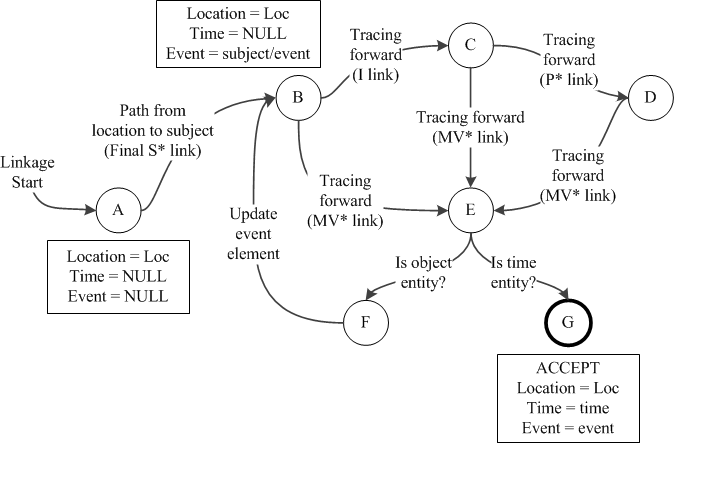
\includegraphics[scale=0.5]{flow_diagram.png}
 \begin{center}
  {\bf Figure 2} : A rough flow diagram for the analysis of each linkage.
 \end{center}
 
  \section{Experiments and Results}
 Here is a sample list of sentence types that our algorithm handles. The Notation A/B for a word is used where A is the actual word, and B is the 
 corresponding Named Entity Tag.
 \begin{itemize}
  \item The party begins in California/location at 5/time AM/time. - \textit{location\_time(party.n, California, 5 AM)}
 \item The party will happen in California/location at 5/time AM/time. - \textit{location\_time(party.n, California, 5 AM)}
 \item The party will be happening in California/location at 5/time AM/time. - \textit{location\_time(party.n, California, 5 AM)}
 \item We conduct the party/OBJECT in California/location on Fridays/time. - \textit{location\_time(party.n, California, Fridays)}
 \item We will be conducting the party in California/location on Fridays/time. - \textit{location\_time(party.n, California, Fridays)}
  \item The meeting with the Professor is scheduled at 9/time AM/time in BSB/location. - \textit{location\_time(meeting.n, BSB, 9 AM)}
  \item The Professor will meet you in BSB/location at 9/time AM/time. - \textit{location\_time(you, BSB, 9 AM)}
  \item An earthquake has been reported in Ohio/location at 4/time AM/time. - \textit{location\_time(earthquake.n, Ohio, 4 AM)}

 \end{itemize}
 
%  The first three sentences output \textit{location\_time(party.n, California, 5 AM) }, and the last two output \textit{location\_time(party.n, California, Fridays) }

%  Now the most important question arises. What is the advantage of using Link Grammars over other types of grammars? 
%  The main advantage of using Link grammars in this context is that they can effectively establish/break relationship between the unrelated subject and 
%  object words, especially in case of conjunctions. The party begins in California at 5 AM 
 
 
\section{Conclusion and Future Work}
We have shown the capabilities of a link grammar in relation extraction by demonstrating a simple location-time relation extraction mechanism with the link parser.
Link grammars are easy to describe, provide the right level of abstraction for semantic analysis in terms of the links, and hence demonstrate substantial 
power for in-depth analysis of sentences. 

With respect to future work, we have the following ideas in mind. Currently, our evaluation measure is purely
subjective. As an objective evaluation measure, we would like to work on a dataset with sentences labeled with the corresponding location-time relation(if existing), and then 
 evaluate precision and recall measures of our algorithm on the dataset. We would also like to extend our algorithm to support more complex location-time 
 relations, for example \textit{The party happens in California/location and Michigan/location at 10/time AM/time and 11/time AM/time respectively}. We would then also like to build a google app that integrates itself into gmail, to automatically establish these relations
 from email sentences, which also automatically adds them to the user's google calendar.
%  \end{figure}

%  \end{center}
\bibliography{references.bib}
 


 
 

\end{document}
